\documentclass[
  bibliography=totoc,     % Literatur im Inhaltsverzeichnis
  captions=tableheading,  % Tabellenüberschriften
  titlepage=firstiscover, % Titelseite ist Deckblatt
]{scrartcl}

\parindent0pt

% Paket float verbessern
\usepackage{scrhack}

% Warnung, falls nochmal kompiliert werden muss
\usepackage[aux]{rerunfilecheck}

% deutsche Spracheinstellungen
\usepackage{polyglossia}
\setmainlanguage{german}

% unverzichtbare Mathe-Befehle
\usepackage{amsmath}
% viele Mathe-Symbole
\usepackage{amssymb}
% Erweiterungen für amsmath
\usepackage{mathtools}

% Fonteinstellungen
\usepackage{fontspec}
% Latin Modern Fonts werden automatisch geladen

\usepackage{csvsimple}

\usepackage[
  math-style=ISO,    % ┐
  bold-style=ISO,    % │
  sans-style=italic, % │ ISO-Standard folgen
  nabla=upright,     % │
  partial=upright,   % ┘
  warnings-off={           % ┐
    mathtools-colon,       % │ unnötige Warnungen ausschalten
    mathtools-overbracket, % │
  },                       % ┘
]{unicode-math}

% traditionelle Fonts für Mathematik
\setmathfont{Latin Modern Math}
\setmathfont{XITS Math}[range={scr, bfscr}]
\setmathfont{XITS Math}[range={cal, bfcal}, StylisticSet=1]

% Zahlen und Einheiten
\usepackage[
  locale=DE,                 % deutsche Einstellungen
  separate-uncertainty=true, % immer Fehler mit \pm
  per-mode=reciprocal,       % ^-1 für inverse Einheiten
  output-decimal-marker=.,   % . statt , für Dezimalzahlen
]{siunitx}

% chemische Formeln
\usepackage[
  version=4,
  math-greek=default, % ┐ mit unicode-math zusammenarbeiten
  text-greek=default, % ┘
]{mhchem}

% richtige Anführungszeichen
\usepackage[autostyle]{csquotes}

% schöne Brüche im Text
\usepackage{xfrac}

% Standardplatzierung für Floats einstellen
\usepackage{float}
\floatplacement{figure}{htbp}
\floatplacement{table}{htbp}
\restylefloat{figure}
% Floats innerhalb einer Section halten
\usepackage[
  section, % Floats innerhalb der Section halten
  below,   % unterhalb der Section aber auf der selben Seite ist ok
]{placeins}

% Seite drehen für breite Tabellen
\usepackage{pdflscape}

% Captions schöner machen.
\usepackage[
  labelfont=bf,        % Tabelle x: Abbildung y: ist jetzt fett
  font=small,          % Schrift etwas kleiner als Dokument
  width=0.9\textwidth, % maximale Breite einer Caption schmaler
]{caption}
% subfigure, subtable, subref
\usepackage{subcaption}

% Grafiken können eingebunden werden
\usepackage{graphicx}
% größere Variation von Dateinamen möglich
\usepackage{grffile}

% schöne Tabellen
\usepackage{booktabs}

% Verbesserungen am Schriftbild
\usepackage{microtype}

% Literaturverzeichnis
\usepackage[
  backend=biber,
]{biblatex}
% Quellendatenbank
\addbibresource{lit.bib}


% Hyperlinks im Dokument
\usepackage[
  unicode,        % Unicode in PDF-Attributen erlauben
  pdfusetitle,    % Titel, Autoren und Datum als PDF-Attribute
  pdfcreator={},  % ┐ PDF-Attribute säubern
  pdfproducer={}, % ┘
]{hyperref}
% erweiterte Bookmarks im PDF
\usepackage{bookmark}

% Trennung von Wörtern mit Strichen
\usepackage[shortcuts]{extdash}

\author{
  Lukas Nickel
  \texorpdfstring{
    \\
    \href{mailto:lukas.nickel@tu-dortmund.de}{lukas.nickel@tu-dortmund.de}
  }{}%
  \texorpdfstring{\and}{, }
  Rohat Kavili
  \texorpdfstring{
    \\
    \href{mailto:rohat.kavili@tu-dortmund.de}{rohat.kavili@tu-dortmund.de}
  }{}%
}
\publishers{TU Dortmund – Fakultät Physik}


\title{SMD Übungsblatt2 - Barth, Kaiser, Nickel}

\begin{document}

\section{Aufgabe 9}
\subsection{a)}
Für a werden ganzzahlige Werte von 1 bis 20 genutzt.
Dabei zeigt sich, dass die Periodenlänge maximal wird für 
a-1 teilbar durch 2 (Primfaktor von 1024) und 4. 

\begin{figure}[H]
  \centering
  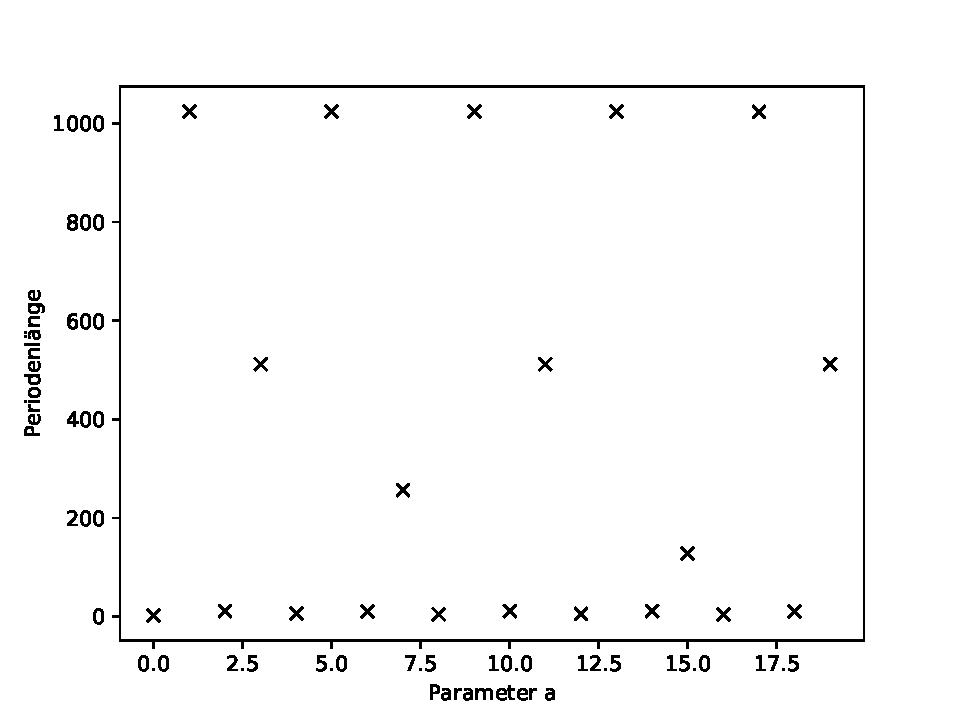
\includegraphics[width=0.8\textwidth]{nr8_a.pdf}
  \caption{Periodenlänge für b=3, m=1024}
  % \label{fig:501200}
\end{figure}


\subsection{b)}
Ok, wird gemacht :)

\subsection{c)}
Die Histogramme sehen alle gleich aus.
Allerdings werden abhängig vom Seed 625 unterschiedliche 
Zahlen (entsprechend Periodenlänge 625) generiert, für genug Bins sollte 
man daher einen Unterschied erkennen (Wird dann allerdings 
schnell unübersichtlich.)
(Mit pl=True bricht der RNG im Script 
nach einer Periode ab.)

\begin{figure}[H]
  \centering
  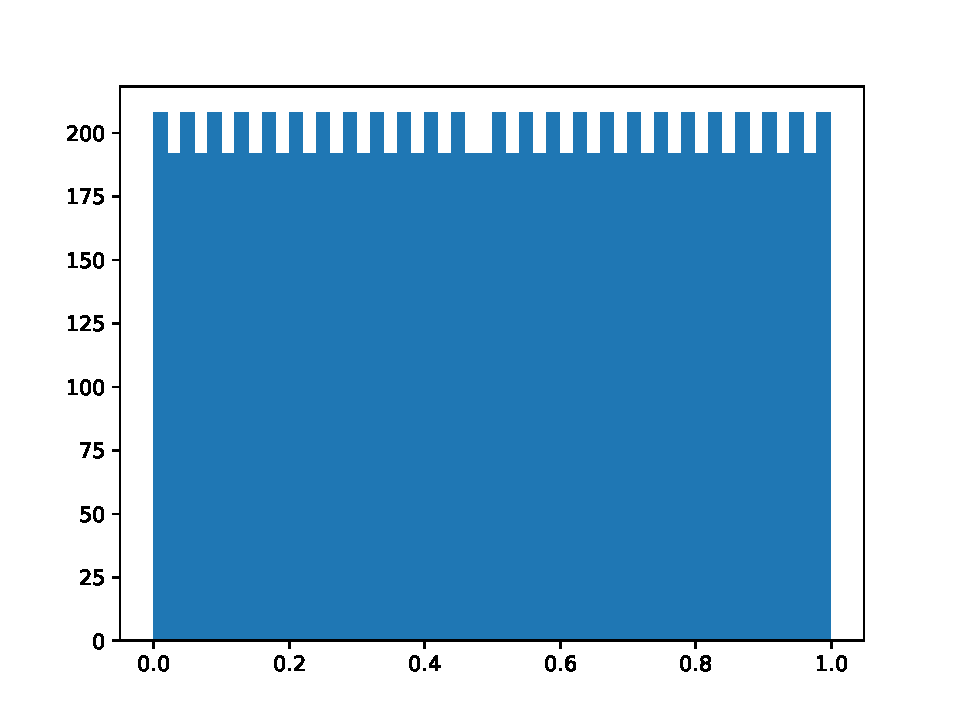
\includegraphics[width=0.8\textwidth]{nr8_c_seed=0.0.pdf}
  \caption{Histogramm für seed = 0.0}
\end{figure}

\begin{figure}[H]
  \centering
  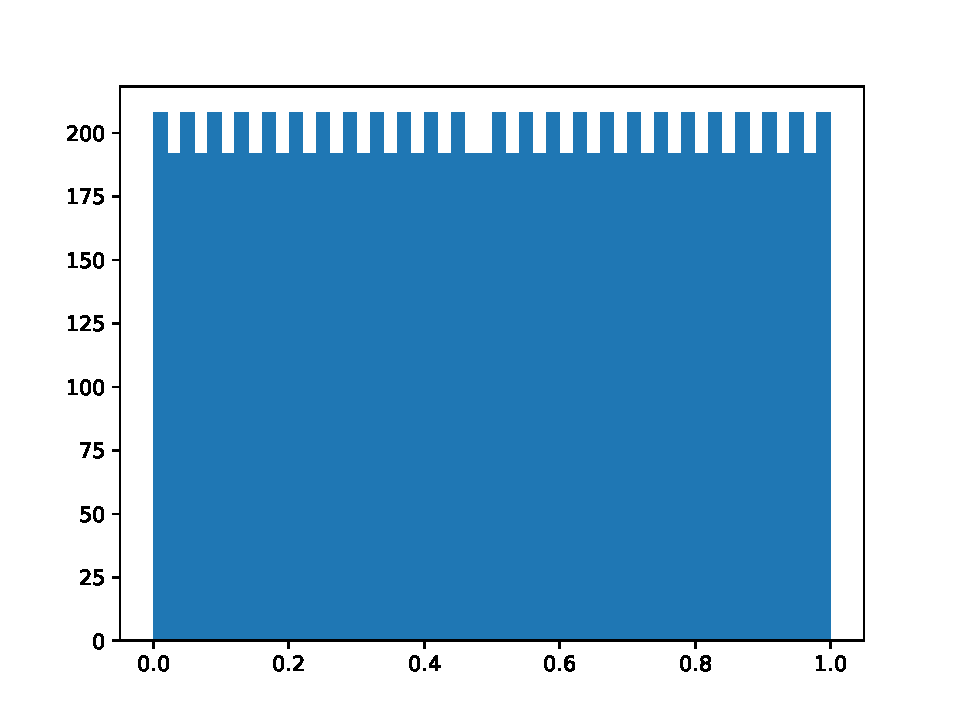
\includegraphics[width=0.8\textwidth]{nr8_c_seed=0.1.pdf}
  \caption{Histogramm für seed = 0.1}
\end{figure}

\begin{figure}[H]
  \centering
  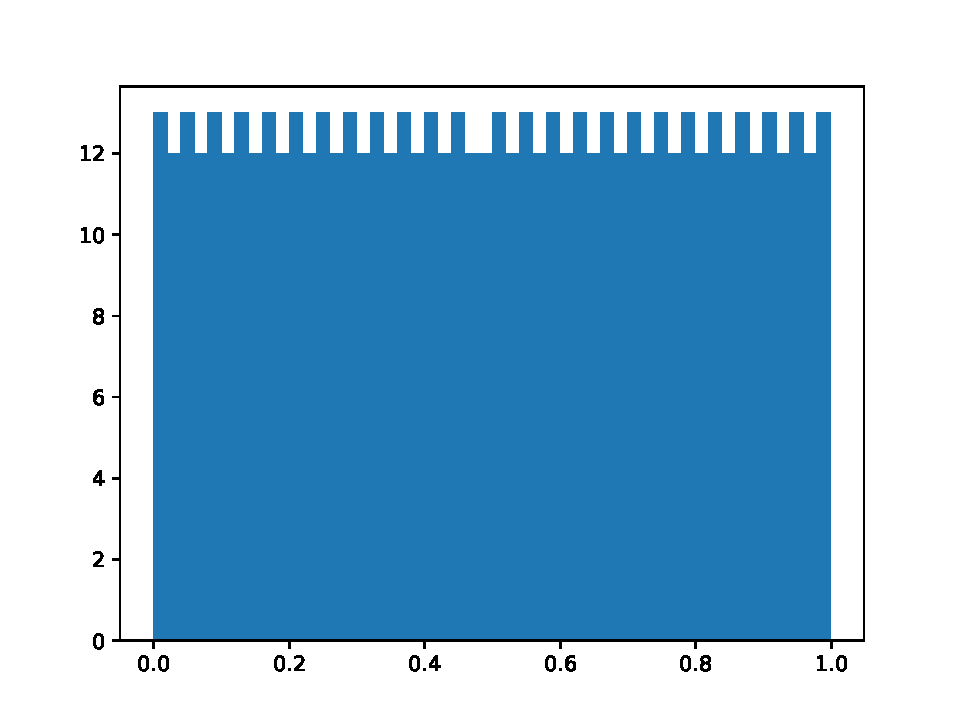
\includegraphics[width=0.8\textwidth]{nr8_c_seed=0.2.pdf}
  \caption{Histogramm für seed = 0.2}
\end{figure}

\begin{figure}[H]
  \centering
  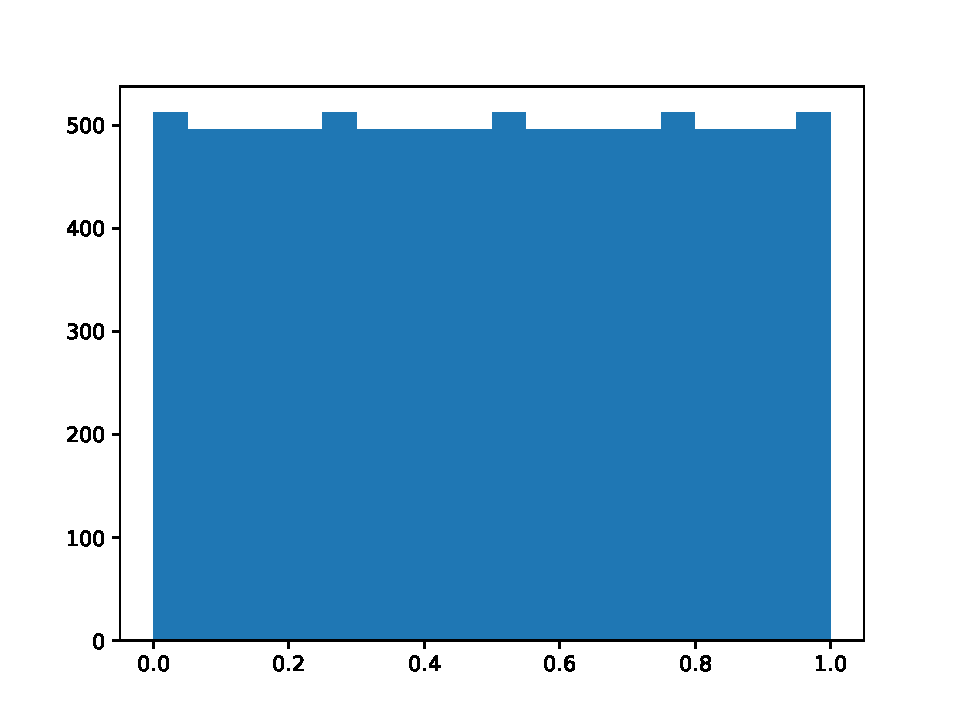
\includegraphics[width=0.8\textwidth]{nr8_c_seed=0.3.pdf}
  \caption{Histogramm für seed = 0.3}
\end{figure}

\begin{figure}[H]
  \centering
  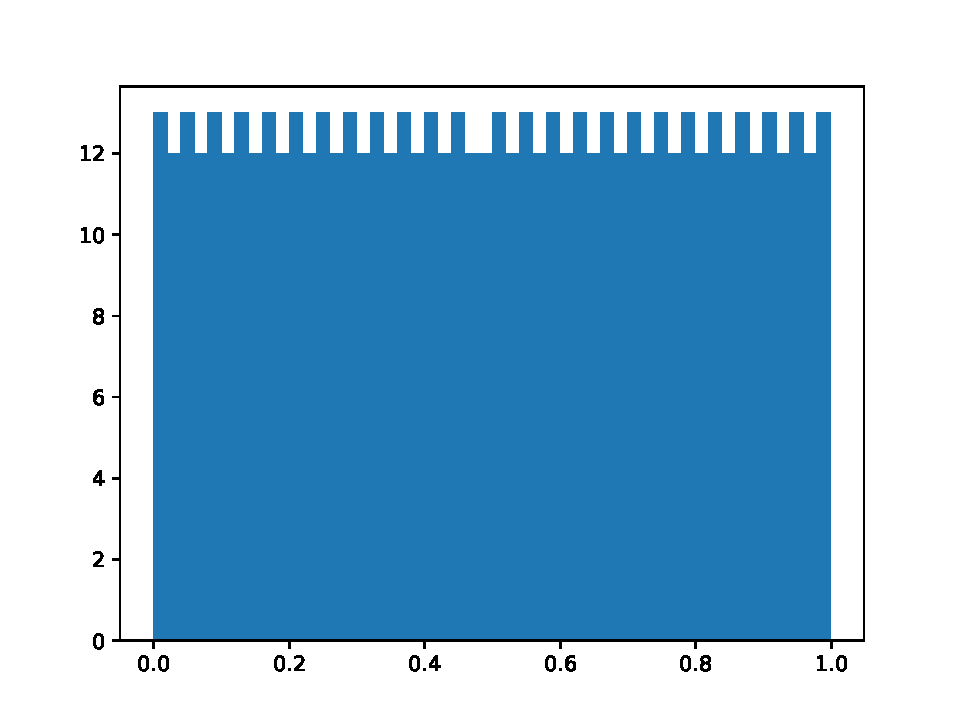
\includegraphics[width=0.8\textwidth]{nr8_c_seed=0.4.pdf}
  \caption{Histogramm für seed = 0.4}
\end{figure}

\begin{figure}[H]
  \centering
  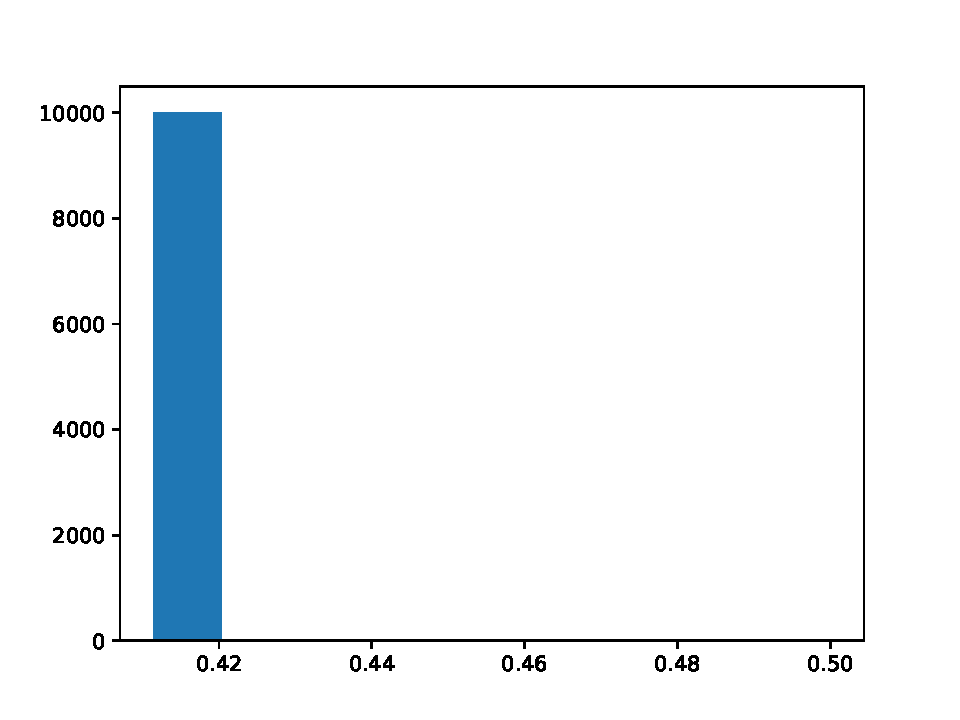
\includegraphics[width=0.8\textwidth]{nr8_c_seed=0.5.pdf}
  \caption{Histogramm für seed = 0.5}
\end{figure}

\begin{figure}[H]
  \centering
  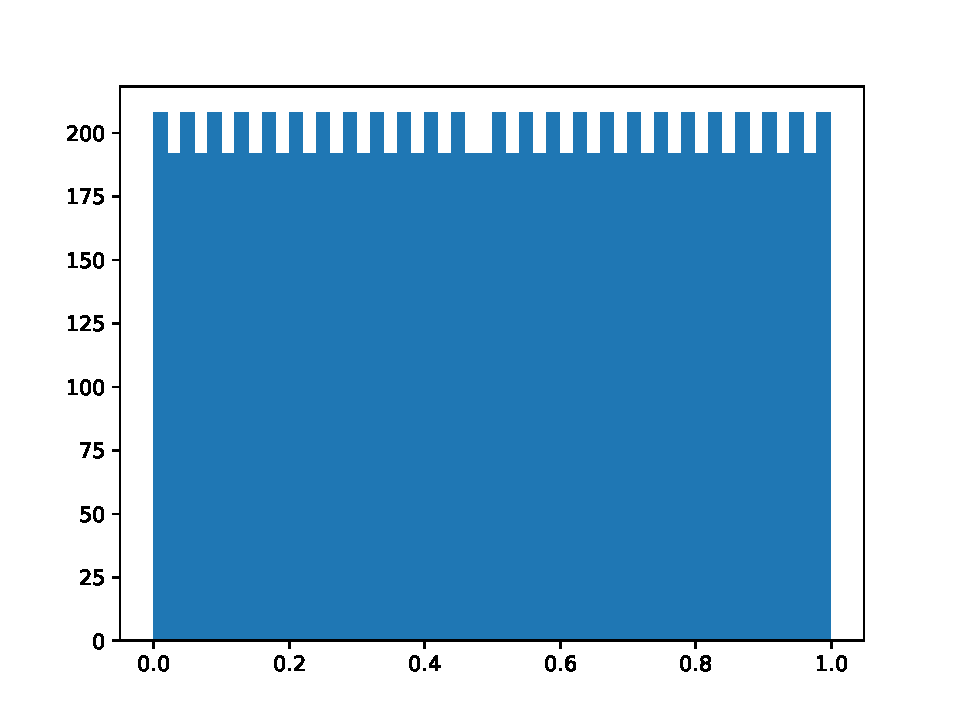
\includegraphics[width=0.8\textwidth]{nr8_c_seed=0.6.pdf}
  \caption{Histogramm für seed = 0.6}
\end{figure}

\begin{figure}[H]
  \centering
  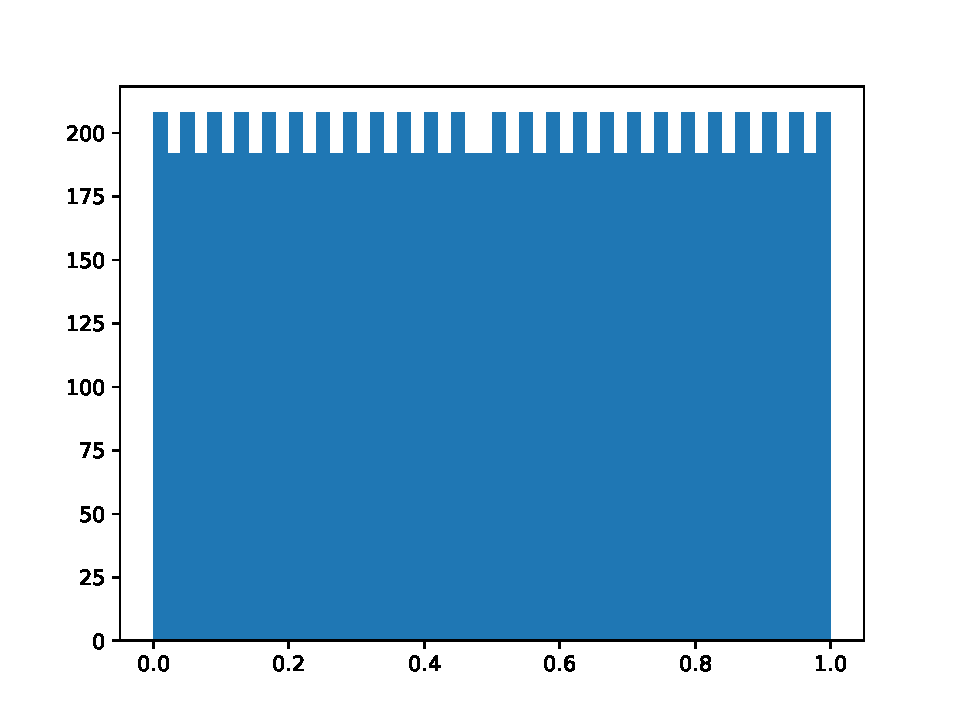
\includegraphics[width=0.8\textwidth]{nr8_c_seed=0.7.pdf}
  \caption{Histogramm für seed = 0.7}
\end{figure}

\begin{figure}[H]
  \centering
  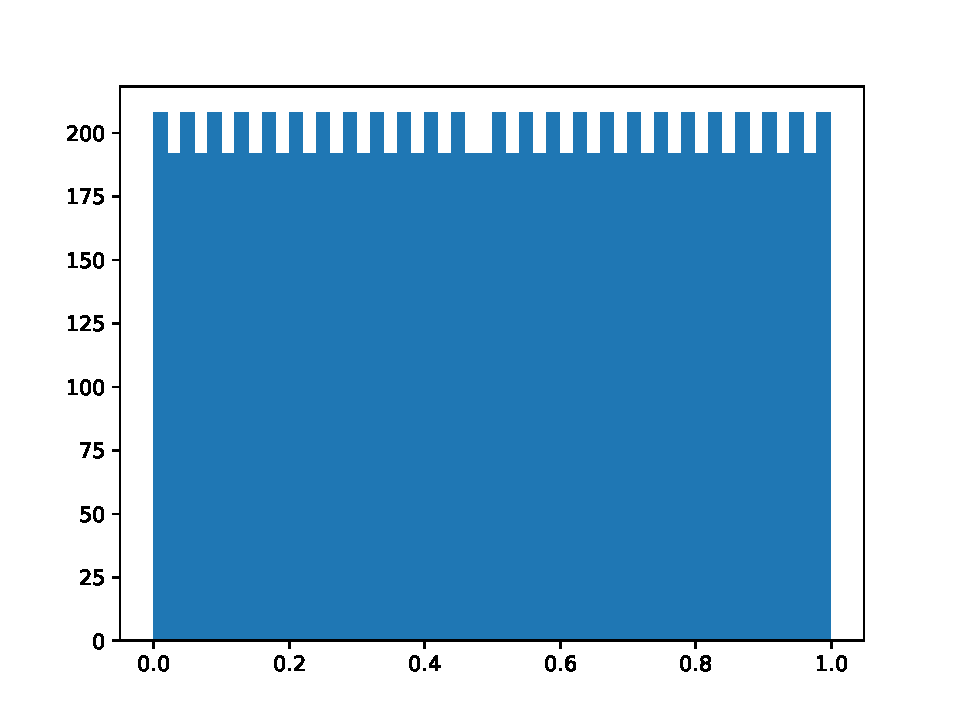
\includegraphics[width=0.8\textwidth]{nr8_c_seed=0.8.pdf}
  \caption{Histogramm für seed = 0.8}
\end{figure}

\begin{figure}[H]
  \centering
  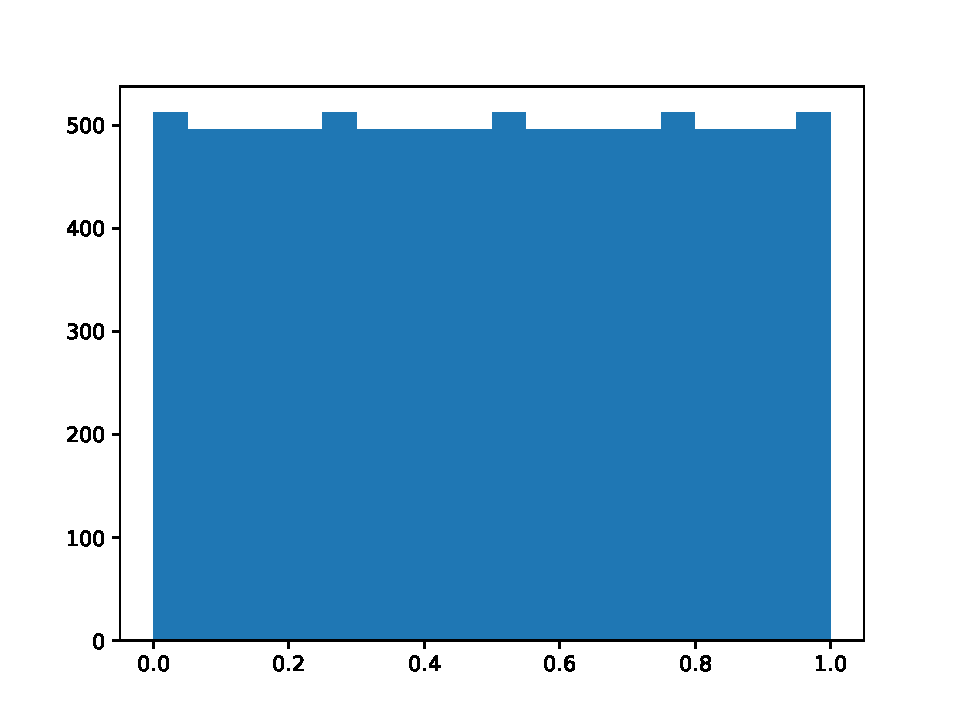
\includegraphics[width=0.8\textwidth]{nr8_c_seed=0.9.pdf}
  \caption{Histogramm für seed = 0.9}
\end{figure}

\subsection{d), e)}
Exemplarisch für Seed = 0.2:

\begin{figure}[H]
  \centering
  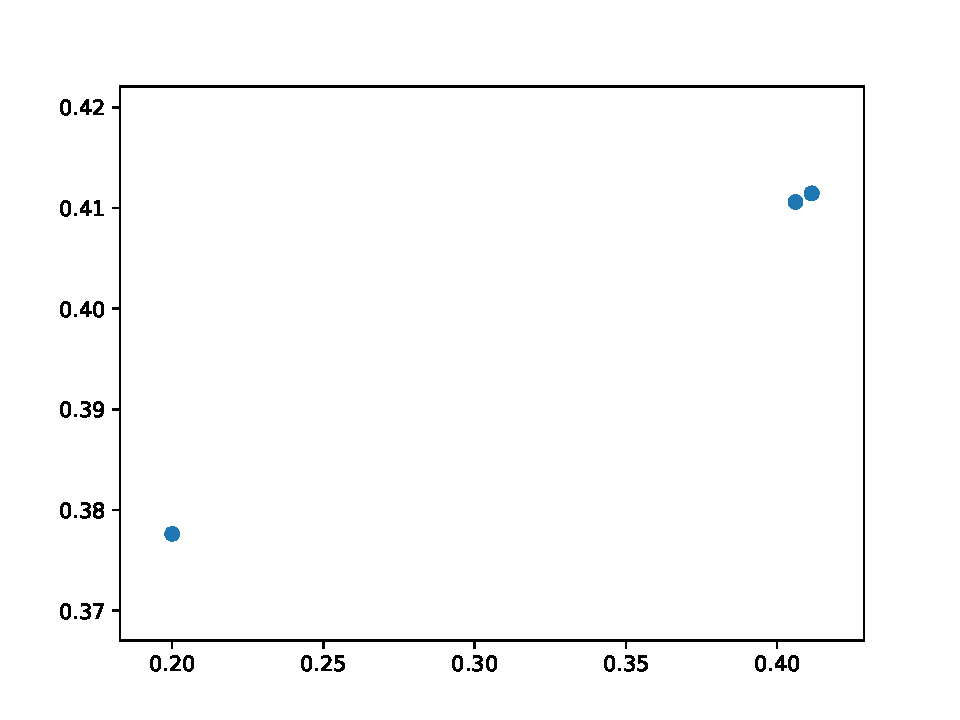
\includegraphics[width=0.8\textwidth]{nr8_d_2D_seed=0.2.pdf}
  \caption{2D Histogramm mit konstruiertem RNG}
\end{figure}

\begin{figure}[H]
  \centering
  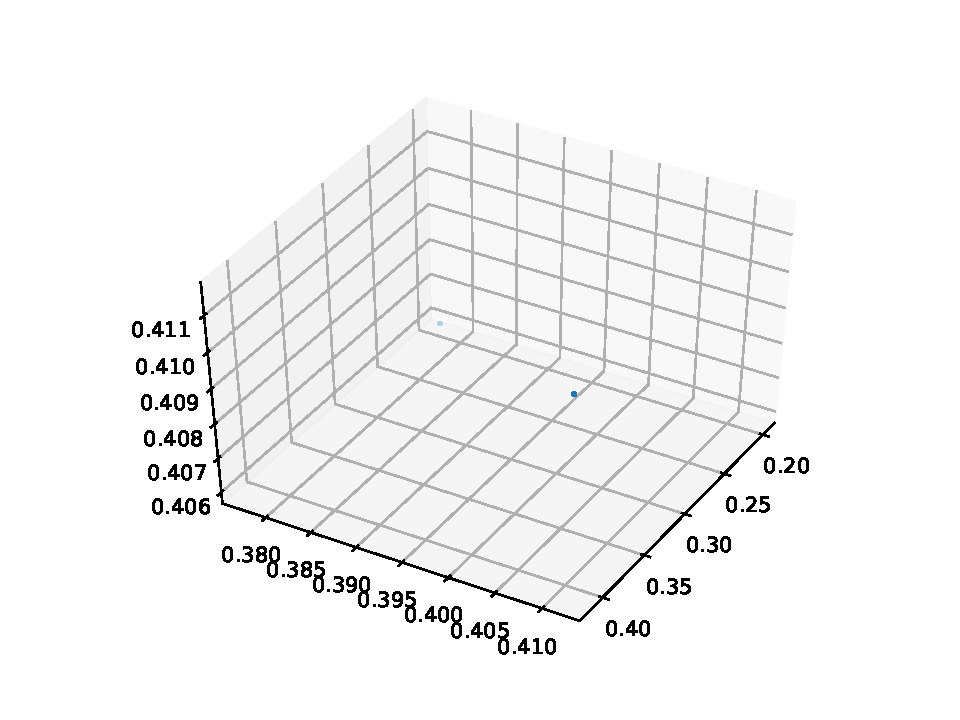
\includegraphics[width=0.8\textwidth]{nr8_d_3D_seed=0.2.pdf}
  \caption{3D Histogramm mit konstruiertem RNG}
\end{figure}

\begin{figure}[H]
  \centering
  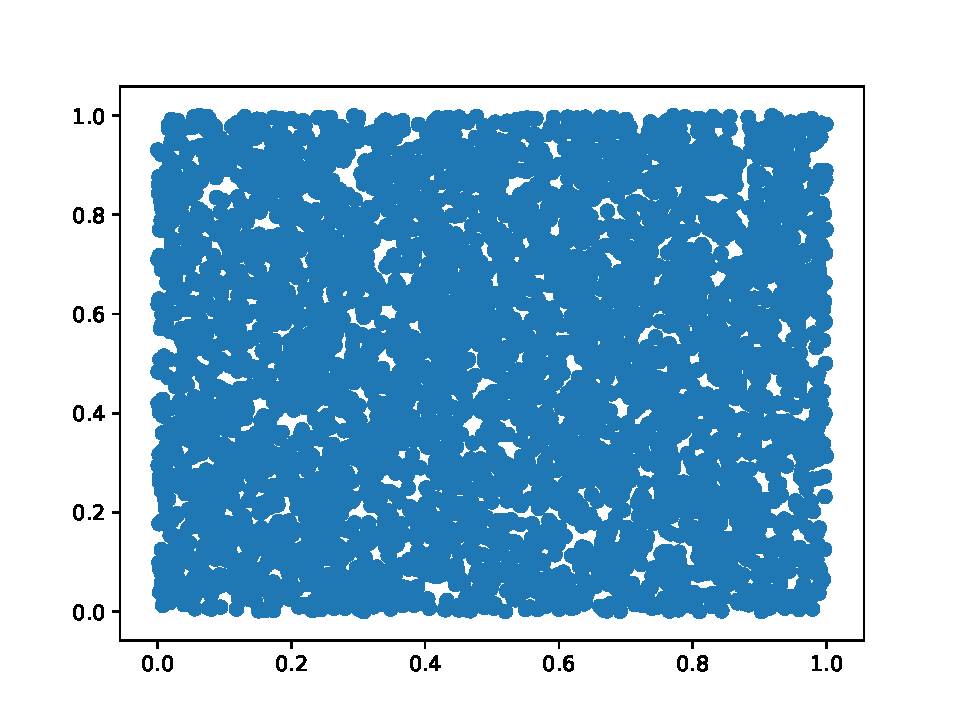
\includegraphics[width=0.8\textwidth]{nr8_d_npuni_2D_seed=0.2.pdf}
  \caption{2D Histogramm mit numpy.random.uniform()}
\end{figure}

\begin{figure}[H]
  \centering
  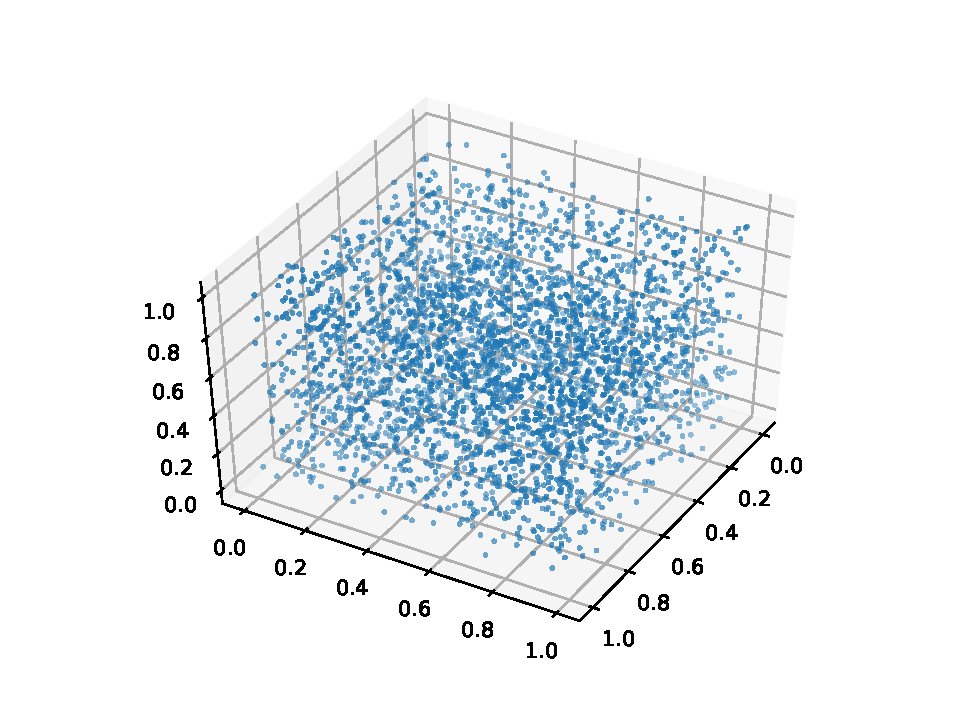
\includegraphics[width=0.8\textwidth]{nr8_d_npuni_3D_seed=0.2.pdf}
  \caption{3D Histogramm mit numpy.random.uniform()}
\end{figure}


Nein, ein guter Zufallsgenerator würde mehr Hyperebenen erzeugen.
Bei 625 generierten Zahlen wären im 
3D Histogramm bis zu $(625)^{1/3} \approx 8.5$ Ebenen
möglich. (Stimmt das so? Die Formel tauchte bei Spektraltest
irgendwo im Internet auf...)
Bei Numpy.Uniform lassen sich sehr viel schlechter Strukturen erkennen, 
wodurch dieser RNG deutlich besser als der linear kongruente mit 
den gegebenen Parametern ist. 
\subsection{f)}

1/2 findet sich abhängig vom Seed 16mal oder 0mal
in den 10000 generierten Zufallszahlen.
In den vorherigen Aufgaben hatte sich gezeigt, dass 
die Periodenlänge mit diesen Parametern 625 beträgt.
Daher wird jede generierte Zahl in den 10000
Werten 16mal zu finden sein (625*16=10000).

\begin{figure}[H]
  \centering
  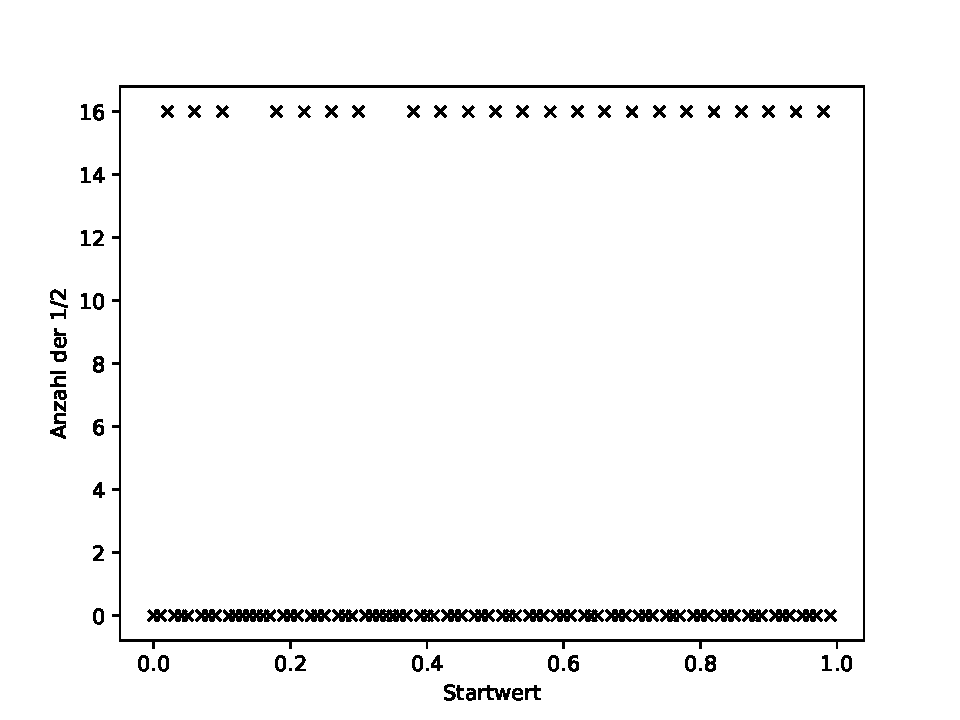
\includegraphics[width=0.8\textwidth]{nr8_f.pdf}
  \caption{Anzahl der 1/2 in 10000 Zufallszahlen}
\end{figure}

\end{document}

